\documentclass[11pt, a4paper]{article}

% Fonts and Encoding
\usepackage[utf8]{inputenc}
\usepackage[T1]{fontenc}

% Math and Symbols
\usepackage{amsmath, amssymb, amsthm, amsfonts, mathrsfs, mathtools}

% Layout and Geometry
\usepackage{geometry}
\geometry{a4paper, margin=1in}

% Formatting and Graphics
\usepackage{graphicx, xcolor, enumitem, booktabs, array, tabularx}

% TikZ for Illustrations
\usepackage{tikz}
\usetikzlibrary{arrows.meta, positioning, shapes.geometric, calc, backgrounds, matrix}

% Clickable Links and TOC
\usepackage{hyperref}
\hypersetup{
    colorlinks=true,
    linkcolor=blue,
    filecolor=magenta,      
    urlcolor=cyan,
    pdftitle={Advanced Mathematics Topic},
}

% Theorem Environments
\newtheorem{theorem}{Theorem}[section]
\newtheorem{lemma}[theorem]{Lemma}
\newtheorem{proposition}[theorem]{Proposition}
\newtheorem{corollary}[theorem]{Corollary}
\theoremstyle{definition}
\newtheorem{definition}{Definition}[section]
\newtheorem{axiom}{Axiom}[section]
\newtheorem{example}{Example}[section]
\theoremstyle{remark}
\newtheorem{remark}{Remark}[section]

% Custom Commands (Enforced standard notation)
\newcommand{\R}{\mathbb{R}}
\newcommand{\N}{\mathbb{N}}
\newcommand{\Z}{\mathbb{Z}}
\newcommand{\Q}{\mathbb{Q}}
\newcommand{\E}{\mathbb{E}}
\newcommand{\Prob}{\mathbb{P}}
\newcommand{\F}{\mathcal{F}}

\begin{document}

\title{\textbf{Advanced Abstract Mathematics: \\ The Expected Value and Variance of Linear Functions of Random Variables}}
\author{Tashfeen Omran}
\date{\today}

\maketitle
\tableofcontents
\newpage

\section{Part 1: Comprehensive Introduction, Context, and Prerequisites}

\subsection{Core Concepts \& Axioms}
In the rigorous study of probability theory, random variables are not merely "unknown quantities" but are formally defined as measurable functions mapping a sample space $\Omega$ to the real numbers $\R$. When modeling complex stochastic systems, we frequently encounter scenarios where the quantity of interest is a linear combination of several underlying random variables. 

Let $Y_1, Y_2, \dots, Y_n$ be random variables defined on a common probability space $(\Omega, \F, \Prob)$. A linear function (or linear combination) of these variables is defined as:
\[ U = \sum_{i=1}^n a_i Y_i \]
where $a_1, a_2, \dots, a_n \in \R$ are deterministic scalar constants. The fundamental objective of this topic is to derive the expected value (first moment) and variance (second central moment) of $U$ strictly in terms of the marginal moments and pairwise covariances of the constituent variables $Y_i$.

\subsection{Intuition and Set-Theoretic/Logical Foundations}
From a measure-theoretic perspective, the expected value is a Lebesgue integral with respect to the probability measure $\Prob$:
\[ \E[Y] = \int_{\Omega} Y(\omega) \, d\Prob(\omega) \]
Because the Lebesgue integral is a linear operator, the expectation of a linear combination is simply the linear combination of the expectations. This is a profound structural property: expectation preserves the vector space structure of random variables.

Variance, however, is a non-linear operator. It measures the expected squared deviation from the mean. When we square a sum, cross-terms emerge. These cross-terms represent the \textit{covariance} between pairs of variables, capturing how they co-vary or move together across the sample space. If two variables are independent, their joint probability measure factors into the product of their marginal measures, causing the covariance cross-terms to vanish.

\subsection{Historical Context and Motivation}
The formalization of these properties traces back to Andrey Kolmogorov's 1933 axiomatization of probability theory. Before this, statisticians struggled to rigorously justify why the variance of a sum of dependent variables required a correction factor. In applied fields like physics (statistical mechanics) and later in quantitative finance (Harry Markowitz's Modern Portfolio Theory in 1952), understanding the variance of linear combinations became the mathematical bedrock for minimizing risk and understanding macroscopic variance arising from microscopic interactions.

\subsection{Key Theorems, Lemmas, and Formulas}
\begin{theorem}[Linearity of Expectation and Variance of Sums]
Let $Y_1, Y_2, \dots, Y_n$ and $X_1, X_2, \dots, X_m$ be random variables with finite second moments. Let $U_1 = \sum_{i=1}^n a_i Y_i$ and $U_2 = \sum_{j=1}^m b_j X_j$. Then:
\begin{enumerate}
    \item \textbf{Expectation:} $\E[U_1] = \sum_{i=1}^n a_i \E[Y_i]$
    \item \textbf{Variance:} $V(U_1) = \sum_{i=1}^n a_i^2 V(Y_i) + 2 \sum_{1 \le i < j \le n} a_i a_j \text{Cov}(Y_i, Y_j)$
    \item \textbf{Covariance:} $\text{Cov}(U_1, U_2) = \sum_{i=1}^n \sum_{j=1}^m a_i b_j \text{Cov}(Y_i, X_j)$
\end{enumerate}
\end{theorem}

\subsection{Prerequisites}
To fully master this chapter, the reader must possess:
\begin{itemize}
    \item \textbf{Measure Theory Basics:} Understanding random variables as measurable functions.
    \item \textbf{Multivariate Calculus:} Proficiency in evaluating double and triple integrals over constrained geometric regions.
    \item \textbf{Foundational Probability:} Mastery of marginal distributions, joint density functions, and the definitions of covariance and correlation.
\end{itemize}

\newpage
\section{Part 2: Detailed Homework Solutions}

\subsection{Exercise 5.102}
\textbf{Problem:} A firm purchases two types of industrial chemicals. Type I costs \$3 per gallon, Type II costs \$5 per gallon. The mean and variance for gallons of Type I, $Y_1$, are 40 and 4. For Type II, $Y_2$, $\E[Y_2] = 65$ and $V(Y_2) = 8$. Assume $Y_1$ and $Y_2$ are independent. Find the mean and variance of the total amount of money spent per week.

\textbf{Solution:}
Let $C$ be the total cost. We can express $C$ as a linear combination of the random variables:
\[ C = 3Y_1 + 5Y_2 \]
By the linearity of expectation (Theorem 5.12a):
\begin{align*}
\E[C] &= \E[3Y_1 + 5Y_2] \\
&= 3\E[Y_1] + 5\E[Y_2] \\
&= 3(40) + 5(65) \\
&= 120 + 325 = 445
\end{align*}
Since $Y_1$ and $Y_2$ are independent, their covariance is zero. By Theorem 5.12b:
\begin{align*}
V(C) &= V(3Y_1 + 5Y_2) \\
&= 3^2 V(Y_1) + 5^2 V(Y_2) \\
&= 9(4) + 25(8) \\
&= 36 + 200 = 236
\end{align*}
\textbf{Conclusion:} The expected total cost is \$445, and the variance is 236. $\blacksquare$

\subsection{Exercise 5.103}
\textbf{Problem:} Assume $Y_1, Y_2, Y_3$ are random variables with $\E[Y_1]=2, \E[Y_2]=-1, \E[Y_3]=4$, $V(Y_1)=4, V(Y_2)=6, V(Y_3)=8$, $\text{Cov}(Y_1,Y_2)=1, \text{Cov}(Y_1,Y_3)=-1, \text{Cov}(Y_2,Y_3)=0$. Find $\E[3Y_1 + 4Y_2 - 6Y_3]$ and $V(3Y_1 + 4Y_2 - 6Y_3)$.

\textbf{Solution:}
Let $U = 3Y_1 + 4Y_2 - 6Y_3$.
Using linearity of expectation:
\begin{align*}
\E[U] &= 3\E[Y_1] + 4\E[Y_2] - 6\E[Y_3] \\
&= 3(2) + 4(-1) - 6(4) \\
&= 6 - 4 - 24 = -22
\end{align*}
Using the variance of a linear combination (Theorem 5.12b):
\begin{align*}
V(U) &= 3^2 V(Y_1) + 4^2 V(Y_2) + (-6)^2 V(Y_3) \\
&\quad + 2(3)(4)\text{Cov}(Y_1,Y_2) + 2(3)(-6)\text{Cov}(Y_1,Y_3) + 2(4)(-6)\text{Cov}(Y_2,Y_3) \\
&= 9(4) + 16(6) + 36(8) + 24(1) - 36(-1) - 48(0) \\
&= 36 + 96 + 288 + 24 + 36 - 0 \\
&= 480
\end{align*}
\textbf{Conclusion:} $\E[U] = -22$ and $V(U) = 480$. $\blacksquare$

\subsection{Exercise 5.104}
\textbf{Problem:} The joint probability distribution of $Y_1$ (married executives) and $Y_2$ (never-married executives) is given by $p(y_1, y_2) = \binom{4}{y_1}\binom{3}{y_2}\binom{2}{3-y_1-y_2} / \binom{9}{3}$.
a) Find $\E[Y_1+Y_2]$ and $V(Y_1+Y_2)$ by first finding the probability distribution of $Y_1+Y_2$.
b) In Ex 5.90, $\text{Cov}(Y_1,Y_2) = -1/3$. Find $\E[Y_1+Y_2]$ and $V(Y_1+Y_2)$ using Theorem 5.12.

\textbf{Solution:}
\textbf{Part a:} Let $W = Y_1 + Y_2$. The experiment involves selecting $n=3$ executives from a total of $N=9$. The pool consists of 4 married, 3 never-married, and 2 "other" executives. The variable $W$ represents the total number of executives in the sample who are either married or never-married. The total number of such "success" candidates in the population is $r = 4 + 3 = 7$.
Thus, $W$ follows a hypergeometric distribution with parameters $N=9, r=7, n=3$.
The probability mass function is:
\[ P(W = w) = \frac{\binom{7}{w}\binom{2}{3-w}}{\binom{9}{3}}, \quad w \in \{1, 2, 3\} \]
For a hypergeometric distribution, the mean and variance are known analytically:
\begin{align*}
\E[W] &= n \left(\frac{r}{N}\right) = 3 \left(\frac{7}{9}\right) = \frac{7}{3} \\
V(W) &= n \left(\frac{r}{N}\right) \left(1 - \frac{r}{N}\right) \left(\frac{N-n}{N-1}\right) \\
&= 3 \left(\frac{7}{9}\right) \left(\frac{2}{9}\right) \left(\frac{9-3}{9-1}\right) \\
&= \left(\frac{42}{81}\right) \left(\frac{6}{8}\right) = \left(\frac{14}{27}\right) \left(\frac{3}{4}\right) = \frac{42}{108} = \frac{7}{18}
\end{align*}

\textbf{Part b:} We now use Theorem 5.12. $Y_1$ is hypergeometric ($N=9, r_1=4, n=3$) and $Y_2$ is hypergeometric ($N=9, r_2=3, n=3$).
\begin{align*}
\E[Y_1] &= 3(4/9) = 4/3 \\
\E[Y_2] &= 3(3/9) = 1 \\
\E[Y_1+Y_2] &= 4/3 + 1 = 7/3
\end{align*}
The variances are:
\begin{align*}
V(Y_1) &= 3(4/9)(5/9)(6/8) = 60/108 = 5/9 \\
V(Y_2) &= 3(3/9)(6/9)(6/8) = 54/108 = 1/2
\end{align*}
Given $\text{Cov}(Y_1, Y_2) = -1/3$, we apply Theorem 5.12b:
\begin{align*}
V(Y_1 + Y_2) &= V(Y_1) + V(Y_2) + 2\text{Cov}(Y_1, Y_2) \\
&= \frac{5}{9} + \frac{1}{2} + 2\left(-\frac{1}{3}\right) \\
&= \frac{10}{18} + \frac{9}{18} - \frac{12}{18} = \frac{7}{18}
\end{align*}
\textbf{Conclusion:} Both methods yield $\E[Y_1+Y_2] = 7/3$ and $V(Y_1+Y_2) = 7/18$. $\blacksquare$

\subsection{Exercise 5.105}
\textbf{Problem:} $f(y_1, y_2) = 4y_1 y_2$ for $0 \le y_1 \le 1, 0 \le y_2 \le 1$. $Y_1$ and $Y_2$ are independent, $\E[Y_1 - Y_2] = 0$. Find $V(Y_1 - Y_2)$.

\textbf{Solution:}
Since $Y_1$ and $Y_2$ are independent, $\text{Cov}(Y_1, Y_2) = 0$.
The marginal density of $Y_1$ is:
\[ f_1(y_1) = \int_0^1 4y_1 y_2 \, dy_2 = 4y_1 \left[ \frac{y_2^2}{2} \right]_0^1 = 2y_1, \quad 0 \le y_1 \le 1 \]
By symmetry, $f_2(y_2) = 2y_2$.
We compute the variance of $Y_1$:
\begin{align*}
\E[Y_1] &= \int_0^1 y_1 (2y_1) \, dy_1 = \int_0^1 2y_1^2 \, dy_1 = \frac{2}{3} \\
\E[Y_1^2] &= \int_0^1 y_1^2 (2y_1) \, dy_1 = \int_0^1 2y_1^3 \, dy_1 = \frac{2}{4} = \frac{1}{2} \\
V(Y_1) &= \E[Y_1^2] - (\E[Y_1])^2 = \frac{1}{2} - \left(\frac{2}{3}\right)^2 = \frac{1}{2} - \frac{4}{9} = \frac{1}{18}
\end{align*}
By symmetry, $V(Y_2) = 1/18$.
Using Theorem 5.12b:
\[ V(Y_1 - Y_2) = V(Y_1) + (-1)^2 V(Y_2) - 2\text{Cov}(Y_1, Y_2) = \frac{1}{18} + \frac{1}{18} - 0 = \frac{1}{9} \]
\textbf{Conclusion:} $V(Y_1 - Y_2) = 1/9$. $\blacksquare$

\subsection{Exercise 5.106}
\textbf{Problem:} $f(y_1, y_2) = 6(1-y_2)$ for $0 \le y_1 \le y_2 \le 1$. We know $\E[Y_1 - 3Y_2] = -5/4$ and $\text{Cov}(Y_1, Y_2) = 1/40$. Find $V(Y_1 - 3Y_2)$.

\textbf{Solution:}
We must first find the marginal variances.
The marginal density of $Y_1$ is:
\[ f_1(y_1) = \int_{y_1}^1 6(1-y_2) \, dy_2 = 6 \left[ y_2 - \frac{y_2^2}{2} \right]_{y_1}^1 = 6 \left( \frac{1}{2} - y_1 + \frac{y_1^2}{2} \right) = 3(1-y_1)^2, \quad 0 \le y_1 \le 1 \]
The moments of $Y_1$ are:
\begin{align*}
\E[Y_1] &= \int_0^1 3y_1(1-y_1)^2 \, dy_1 = 3 \int_0^1 (y_1 - 2y_1^2 + y_1^3) \, dy_1 = 3\left(\frac{1}{2} - \frac{2}{3} + \frac{1}{4}\right) = \frac{1}{4} \\
\E[Y_1^2] &= \int_0^1 3y_1^2(1-y_1)^2 \, dy_1 = 3 \int_0^1 (y_1^2 - 2y_1^3 + y_1^4) \, dy_1 = 3\left(\frac{1}{3} - \frac{2}{4} + \frac{1}{5}\right) = \frac{1}{10} \\
V(Y_1) &= \frac{1}{10} - \left(\frac{1}{4}\right)^2 = \frac{1}{10} - \frac{1}{16} = \frac{3}{80}
\end{align*}
The marginal density of $Y_2$ is:
\[ f_2(y_2) = \int_0^{y_2} 6(1-y_2) \, dy_1 = 6y_2(1-y_2), \quad 0 \le y_2 \le 1 \]
The moments of $Y_2$ are:
\begin{align*}
\E[Y_2] &= \int_0^1 6y_2^2(1-y_2) \, dy_2 = 6\left(\frac{1}{3} - \frac{1}{4}\right) = \frac{1}{2} \\
\E[Y_2^2] &= \int_0^1 6y_2^3(1-y_2) \, dy_2 = 6\left(\frac{1}{4} - \frac{1}{5}\right) = \frac{3}{10} \\
V(Y_2) &= \frac{3}{10} - \left(\frac{1}{2}\right)^2 = \frac{3}{10} - \frac{1}{4} = \frac{1}{20} = \frac{4}{80}
\end{align*}
Now, applying Theorem 5.12b:
\begin{align*}
V(Y_1 - 3Y_2) &= V(Y_1) + (-3)^2 V(Y_2) + 2(1)(-3)\text{Cov}(Y_1, Y_2) \\
&= \frac{3}{80} + 9\left(\frac{4}{80}\right) - 6\left(\frac{1}{40}\right) \\
&= \frac{3}{80} + \frac{36}{80} - \frac{12}{80} = \frac{27}{80}
\end{align*}
\textbf{Conclusion:} $V(Y_1 - 3Y_2) = 27/80$. $\blacksquare$

\subsection{Exercise 5.107}
\textbf{Problem:} $f(y_1, y_2) = 2$ for $0 \le y_1 \le 1, 0 \le y_2 \le 1, 0 \le y_1+y_2 \le 1$. Find $\E[Y_1+Y_2]$ and $V(Y_1+Y_2)$.

\textbf{Solution:}
Let $W = Y_1 + Y_2$. We can find the distribution of $W$ directly using a geometric argument. The joint density is uniform over the triangle with vertices $(0,0), (1,0), (0,1)$.
The cumulative distribution function $F_W(w) = \Prob(Y_1 + Y_2 \le w)$ for $0 \le w \le 1$ is the integral of the density over the region bounded by $y_1+y_2 \le w$. This region is a triangle with base $w$ and height $w$.
\[ F_W(w) = \text{Area} \times \text{Density} = \left(\frac{1}{2} w^2\right) \times 2 = w^2 \]
Differentiating yields the density of $W$:
\[ f_W(w) = \frac{d}{dw} w^2 = 2w, \quad 0 \le w \le 1 \]
Now we compute the moments of $W$:
\begin{align*}
\E[W] &= \int_0^1 w(2w) \, dw = \int_0^1 2w^2 \, dw = \frac{2}{3} \\
\E[W^2] &= \int_0^1 w^2(2w) \, dw = \int_0^1 2w^3 \, dw = \frac{2}{4} = \frac{1}{2} \\
V(W) &= \E[W^2] - (\E[W])^2 = \frac{1}{2} - \left(\frac{2}{3}\right)^2 = \frac{1}{2} - \frac{4}{9} = \frac{1}{18}
\end{align*}
\textbf{Conclusion:} $\E[Y_1+Y_2] = 2/3$ and $V(Y_1+Y_2) = 1/18$. $\blacksquare$

\subsection{Exercise 5.108}
\textbf{Problem:} $f(y_1, y_2) = e^{-y_1}$ for $0 \le y_2 \le y_1 < \infty$. Find $\E[Y_1 - Y_2]$ and $V(Y_1 - Y_2)$. Is it highly likely that a randomly selected customer would spend more than 4 minutes at the service window?

\textbf{Solution:}
Let $U = Y_1 - Y_2$. We perform a bivariate transformation. Let $U = Y_1 - Y_2$ and $V = Y_2$.
The inverse transformation is $y_1 = u + v$ and $y_2 = v$. The Jacobian determinant is:
\[ J = \det \begin{pmatrix} \frac{\partial y_1}{\partial u} & \frac{\partial y_1}{\partial v} \\ \frac{\partial y_2}{\partial u} & \frac{\partial y_2}{\partial v} \end{pmatrix} = \det \begin{pmatrix} 1 & 1 \\ 0 & 1 \end{pmatrix} = 1 \]
The joint density of $U$ and $V$ is:
\[ f_{U,V}(u, v) = f(u+v, v) |J| = e^{-(u+v)} = e^{-u} e^{-v} \]
The support is $0 \le v \le u+v < \infty$, which simplifies to $u \ge 0$ and $v \ge 0$.
Since the joint density factors into $e^{-u}$ and $e^{-v}$, $U$ and $V$ are independent standard exponential random variables.
Thus, $U \sim \text{Exp}(1)$.
\begin{align*}
\E[U] &= 1 \\
V(U) &= 1
\end{align*}
To find the probability of spending more than 4 minutes:
\[ \Prob(U > 4) = \int_4^\infty e^{-u} \, du = e^{-4} \approx 0.0183 \]
\textbf{Conclusion:} $\E[Y_1-Y_2] = 1$, $V(Y_1-Y_2) = 1$. With only a 1.83\% chance, it is \textit{not} highly likely to exceed 4 minutes. $\blacksquare$

\subsection{Exercise 5.109}
\textbf{Problem:} $f(y_1, y_2) = y_1 + y_2$ for $0 \le y_1, y_2 \le 1$. Find the variance of $30Y_1 + 25Y_2$. Give an interval for at least 75\% of the days.

\textbf{Solution:}
First, we find the marginal moments.
\[ f_1(y_1) = \int_0^1 (y_1 + y_2) \, dy_2 = \left[ y_1 y_2 + \frac{y_2^2}{2} \right]_0^1 = y_1 + \frac{1}{2} \]
\begin{align*}
\E[Y_1] &= \int_0^1 y_1\left(y_1 + \frac{1}{2}\right) \, dy_1 = \frac{1}{3} + \frac{1}{4} = \frac{7}{12} \\
\E[Y_1^2] &= \int_0^1 y_1^2\left(y_1 + \frac{1}{2}\right) \, dy_1 = \frac{1}{4} + \frac{1}{6} = \frac{5}{12} \\
V(Y_1) &= \frac{5}{12} - \left(\frac{7}{12}\right)^2 = \frac{60}{144} - \frac{49}{144} = \frac{11}{144}
\end{align*}
By symmetry, $\E[Y_2] = 7/12$ and $V(Y_2) = 11/144$.
Next, we find the covariance:
\begin{align*}
\E[Y_1 Y_2] &= \int_0^1 \int_0^1 y_1 y_2 (y_1 + y_2) \, dy_2 \, dy_1 = \int_0^1 \int_0^1 (y_1^2 y_2 + y_1 y_2^2) \, dy_2 \, dy_1 \\
&= \int_0^1 \left( \frac{y_1^2}{2} + \frac{y_1}{3} \right) \, dy_1 = \frac{1}{6} + \frac{1}{6} = \frac{1}{3} \\
\text{Cov}(Y_1, Y_2) &= \E[Y_1 Y_2] - \E[Y_1]\E[Y_2] = \frac{1}{3} - \left(\frac{7}{12}\right)^2 = \frac{48}{144} - \frac{49}{144} = -\frac{1}{144}
\end{align*}
Let $W = 30Y_1 + 25Y_2$.
\begin{align*}
\E[W] &= 30\left(\frac{7}{12}\right) + 25\left(\frac{7}{12}\right) = \frac{385}{12} \approx 32.083 \\
V(W) &= 30^2 V(Y_1) + 25^2 V(Y_2) + 2(30)(25)\text{Cov}(Y_1, Y_2) \\
&= 900\left(\frac{11}{144}\right) + 625\left(\frac{11}{144}\right) + 1500\left(-\frac{1}{144}\right) \\
&= \frac{9900 + 6875 - 1500}{144} = \frac{15275}{144} \approx 106.076
\end{align*}
To find an interval containing at least 75\% of the probability mass, we use Chebyshev's Inequality: $\Prob(|W - \mu| < 2\sigma) \ge 1 - 1/2^2 = 0.75$.
The standard deviation is $\sigma = \sqrt{15275}/12 \approx 10.30$.
The interval is $\mu \pm 2\sigma = 32.083 \pm 20.60 = [11.48, 52.68]$.
\textbf{Conclusion:} $V(W) = 15275/144$. The interval is $[11.48, 52.68]$. $\blacksquare$

\subsection{Exercise 5.110}
\textbf{Problem:} Suppose $Y_1$ and $Y_2$ have correlation coefficient $\rho = 0.2$. Find the correlation coefficient between:
a) $1 + 2Y_1$ and $3 + 4Y_2$
b) $1 + 2Y_1$ and $3 - 4Y_2$
c) $1 - 2Y_1$ and $3 - 4Y_2$

\textbf{Solution:}
Let $W_1 = a + bY_1$ and $W_2 = c + dY_2$. The covariance is $\text{Cov}(W_1, W_2) = bd\text{Cov}(Y_1, Y_2)$. The standard deviations are $\sigma_{W_1} = |b|\sigma_{Y_1}$ and $\sigma_{W_2} = |d|\sigma_{Y_2}$.
The correlation is:
\[ \rho_{W_1, W_2} = \frac{bd\text{Cov}(Y_1, Y_2)}{|b||d|\sigma_{Y_1}\sigma_{Y_2}} = \frac{bd}{|bd|} \rho_{Y_1, Y_2} = \text{sgn}(bd) \rho_{Y_1, Y_2} \]
a) $b=2, d=4 \implies \text{sgn}(8) = 1 \implies \rho = 0.2$.
b) $b=2, d=-4 \implies \text{sgn}(-8) = -1 \implies \rho = -0.2$.
c) $b=-2, d=-4 \implies \text{sgn}(8) = 1 \implies \rho = 0.2$. $\blacksquare$

\subsection{Exercise 5.111}
\textbf{Problem:} $X \sim N(50, 3^2)$ and $Y \sim \text{Gamma}(\alpha=4, \beta=2)$. $X$ and $Y$ are independent. Find expected value and variance of net daily gain $U = X - Y$. Would you expect it to rise above \$70?

\textbf{Solution:}
For the normal variable $X$: $\E[X] = 50$, $V(X) = 3^2 = 9$.
For the gamma variable $Y$: $\E[Y] = \alpha\beta = 4(2) = 8$, $V(Y) = \alpha\beta^2 = 4(4) = 16$.
\begin{align*}
\E[U] &= \E[X] - \E[Y] = 50 - 8 = 42 \\
V(U) &= V(X) + (-1)^2 V(Y) = 9 + 16 = 25
\end{align*}
The standard deviation of $U$ is $\sigma_U = \sqrt{25} = 5$.
To rise above \$70, $U$ must exceed its mean by $70 - 42 = 28$ dollars.
This is $28 / 5 = 5.6$ standard deviations above the mean. By Chebyshev's inequality, the probability of exceeding 5.6 standard deviations is at most $1 / (5.6)^2 \approx 0.031$.
\textbf{Conclusion:} $\E[U] = 42$, $V(U) = 25$. It is highly unlikely to rise above \$70. $\blacksquare$

\subsection{Exercise 5.112}
\textbf{Problem:} $f(y_1, y_2) = (1/8)y_1 e^{-(y_1+y_2)/2}$ for $y_1, y_2 > 0$. $C = 50 + 2Y_1 + 4Y_2$. Find $\E[C]$ and $V(C)$.

\textbf{Solution:}
The joint density factors into marginals:
\[ f(y_1, y_2) = \left( \frac{1}{4} y_1 e^{-y_1/2} \right) \left( \frac{1}{2} e^{-y_2/2} \right) \]
Thus, $Y_1$ and $Y_2$ are independent.
$Y_1 \sim \text{Gamma}(\alpha=2, \beta=2) \implies \E[Y_1] = 4, V(Y_1) = 8$.
$Y_2 \sim \text{Exp}(\beta=2) \implies \E[Y_2] = 2, V(Y_2) = 4$.
\begin{align*}
\E[C] &= 50 + 2\E[Y_1] + 4\E[Y_2] = 50 + 2(4) + 4(2) = 66 \\
V(C) &= 2^2 V(Y_1) + 4^2 V(Y_2) = 4(8) + 16(4) = 32 + 64 = 96
\end{align*}
\textbf{Conclusion:} $\E[C] = 66$ and $V(C) = 96$. $\blacksquare$

\subsection{Exercise 5.113}
\textbf{Problem:} $W_1 = a + bY_1$ and $W_2 = c + dY_2$. Show $|\rho_{W_1, W_2}| = |\rho_{Y_1, Y_2}|$. Does this explain 5.110?

\textbf{Solution:}
By definition, $\rho_{W_1, W_2} = \frac{\text{Cov}(W_1, W_2)}{\sigma_{W_1} \sigma_{W_2}}$.
Using the properties of covariance and variance:
\begin{align*}
\text{Cov}(a + bY_1, c + dY_2) &= bd\text{Cov}(Y_1, Y_2) \\
\sigma_{W_1} &= \sqrt{b^2 V(Y_1)} = |b|\sigma_{Y_1} \\
\sigma_{W_2} &= \sqrt{d^2 V(Y_2)} = |d|\sigma_{Y_2}
\end{align*}
Substituting these into the correlation formula:
\[ \rho_{W_1, W_2} = \frac{bd\text{Cov}(Y_1, Y_2)}{|b||d|\sigma_{Y_1}\sigma_{Y_2}} = \frac{bd}{|bd|} \rho_{Y_1, Y_2} \]
Taking the absolute value of both sides:
\[ |\rho_{W_1, W_2}| = \left| \frac{bd}{|bd|} \right| |\rho_{Y_1, Y_2}| = (1) |\rho_{Y_1, Y_2}| = |\rho_{Y_1, Y_2}| \]
\textbf{Conclusion:} Yes, this perfectly explains the results in Exercise 5.110, where the magnitude of the correlation remained 0.2 regardless of the signs of the coefficients. $\blacksquare$

\subsection{Exercise 5.114}
\textbf{Problem:} $f_1(y_1) = (1/6)y_1^3 e^{-y_1}$ and $f_2(y_2) = (1/2)e^{-y_2/2}$. $U = Y_1 - Y_2$. Find $\E[U]$ and $V(U)$ assuming independence. Would you expect profit to drop below zero very often?

\textbf{Solution:}
$Y_1$ follows a Gamma distribution with $\alpha=4, \beta=1$. $\E[Y_1] = 4, V(Y_1) = 4$.
$Y_2$ follows an Exponential distribution with $\beta=2$. $\E[Y_2] = 2, V(Y_2) = 4$.
\begin{align*}
\E[U] &= \E[Y_1] - \E[Y_2] = 4 - 2 = 2 \\
V(U) &= V(Y_1) + (-1)^2 V(Y_2) = 4 + 4 = 8
\end{align*}
The standard deviation is $\sigma_U = \sqrt{8} \approx 2.83$.
Zero profit is $2 / 2.83 \approx 0.71$ standard deviations below the mean. Because zero is less than one standard deviation away from the mean, a substantial portion of the probability distribution lies below zero.
\textbf{Conclusion:} $\E[U] = 2, V(U) = 8$. Yes, we expect the profit to drop below zero fairly often. $\blacksquare$

\subsection{Exercise 5.115}
\textbf{Problem:} Coupon collector's problem. $Y = Y_1 + \dots + Y_6$. $Y_i$ is the number of tosses to get the $i$-th distinct face after $i-1$ faces have been observed. Show $\text{Cov}(Y_i, Y_j) = 0$. Find $V(Y)$ and an interval containing $Y$ with probability at least 3/4.

\textbf{Solution:}
\textbf{Part a:} The random variable $Y_i$ represents the waiting time for the first success in a sequence of Bernoulli trials where the probability of success is $p_i = \frac{7-i}{6}$. Because the die tosses are independent, the waiting time for the $i$-th new face is completely independent of how long it took to get the previous faces. Thus, the variables $Y_i$ are mutually independent, which implies $\text{Cov}(Y_i, Y_j) = 0$ for $i \neq j$.

\textbf{Part b:} Each $Y_i$ follows a Geometric distribution with parameter $p_i$. The variance is $V(Y_i) = \frac{1-p_i}{p_i^2}$.
\begin{align*}
p_1 &= 1 \implies V(Y_1) = 0 \\
p_2 &= 5/6 \implies V(Y_2) = \frac{1/6}{25/36} = \frac{6}{25} = 0.24 \\
p_3 &= 4/6 \implies V(Y_3) = \frac{2/6}{16/36} = \frac{12}{16} = 0.75 \\
p_4 &= 3/6 \implies V(Y_4) = \frac{3/6}{9/36} = \frac{18}{9} = 2 \\
p_5 &= 2/6 \implies V(Y_5) = \frac{4/6}{4/36} = \frac{24}{4} = 6 \\
p_6 &= 1/6 \implies V(Y_6) = \frac{5/6}{1/36} = 30
\end{align*}
By Theorem 5.12, $V(Y) = \sum V(Y_i) = 0 + 0.24 + 0.75 + 2 + 6 + 30 = 38.99$.

\textbf{Part c:} We need the mean: $\E[Y] = \sum \frac{1}{p_i} = 1 + 1.2 + 1.5 + 2 + 3 + 6 = 14.7$.
By Chebyshev's inequality, $\Prob(|Y - \mu| < 2\sigma) \ge 1 - 1/4 = 3/4$.
$\sigma = \sqrt{38.99} \approx 6.244$.
The interval is $14.7 \pm 2(6.244) = 14.7 \pm 12.488 = [2.212, 27.188]$. $\blacksquare$

\subsection{Exercise 5.116}
\textbf{Problem:} Explain why $V(Y_1 + Y_2) = V(Y_1 - Y_2)$ if $\text{Cov}(Y_1, Y_2) = 0$.

\textbf{Solution:}
By Theorem 5.12b:
\begin{align*}
V(Y_1 + Y_2) &= V(Y_1) + V(Y_2) + 2\text{Cov}(Y_1, Y_2) \\
V(Y_1 - Y_2) &= V(Y_1) + (-1)^2 V(Y_2) + 2(1)(-1)\text{Cov}(Y_1, Y_2) \\
&= V(Y_1) + V(Y_2) - 2\text{Cov}(Y_1, Y_2)
\end{align*}
If $\text{Cov}(Y_1, Y_2) = 0$, both expressions collapse to $V(Y_1) + V(Y_2)$, making them strictly equal. $\blacksquare$

\subsection{Exercise 5.117}
\textbf{Problem:} Sampling without replacement. $Y_1$ mature females, $Y_2$ mature males. Proportions $p_1, p_2$. Find expressions for $\E[Y_1/n - Y_2/n]$ and $V(Y_1/n - Y_2/n)$.

\textbf{Solution:}
This is a multivariate hypergeometric distribution. The marginals are standard hypergeometric.
$\E[Y_1] = n p_1$ and $\E[Y_2] = n p_2$.
By linearity of expectation:
\[ \E\left[\frac{Y_1}{n} - \frac{Y_2}{n}\right] = \frac{1}{n}\E[Y_1] - \frac{1}{n}\E[Y_2] = p_1 - p_2 \]
The variances and covariance for sampling without replacement are:
\begin{align*}
V(Y_1) &= n p_1 (1-p_1) \frac{N-n}{N-1} \\
V(Y_2) &= n p_2 (1-p_2) \frac{N-n}{N-1} \\
\text{Cov}(Y_1, Y_2) &= -n p_1 p_2 \frac{N-n}{N-1}
\end{align*}
Using Theorem 5.12b:
\begin{align*}
V\left(\frac{Y_1}{n} - \frac{Y_2}{n}\right) &= \frac{1}{n^2} \left[ V(Y_1) + V(Y_2) - 2\text{Cov}(Y_1, Y_2) \right] \\
&= \frac{1}{n^2} \left( \frac{N-n}{N-1} \right) \left[ n p_1(1-p_1) + n p_2(1-p_2) - 2(-n p_1 p_2) \right] \\
&= \frac{1}{n} \left( \frac{N-n}{N-1} \right) \left[ p_1 - p_1^2 + p_2 - p_2^2 + 2p_1 p_2 \right] \\
&= \frac{1}{n} \left( \frac{N-n}{N-1} \right) \left[ p_1 + p_2 - (p_1 - p_2)^2 \right]
\end{align*}
\textbf{Conclusion:} The variance is $\frac{1}{n} \left( \frac{N-n}{N-1} \right) \left[ p_1 + p_2 - (p_1 - p_2)^2 \right]$. $\blacksquare$

\subsection{Exercise 5.118}
\textbf{Problem:} $X_1 \sim \text{Gamma}(50, 2)$ and $X_2 \sim \text{Gamma}(20, 2)$. Independent. Find mean and variance of $X_1+X_2$. Find a value exceeded with probability less than 1/16.

\textbf{Solution:}
\textbf{Part a:}
\begin{align*}
\E[X_1+X_2] &= \E[X_1] + \E[X_2] = 50(2) + 20(2) = 140 \\
V(X_1+X_2) &= V(X_1) + V(X_2) = 50(2^2) + 20(2^2) = 200 + 80 = 280
\end{align*}
\textbf{Part b:} We use Chebyshev's inequality: $\Prob(|X - \mu| \ge k\sigma) \le 1/k^2$.
We want the probability to be less than $1/16$, so we set $1/k^2 = 1/16 \implies k = 4$.
The standard deviation is $\sigma = \sqrt{280} \approx 16.733$.
The threshold value is $\mu + 4\sigma = 140 + 4(16.733) = 140 + 66.93 = 206.93$.
\textbf{Conclusion:} Mean is 140, variance is 280. The value is 206.93. $\blacksquare$

\newpage
\section{Part 3: In-Depth Analysis of Problems and Techniques}

\subsection{A) Problem Types and Logical Strategies}
\begin{itemize}
    \item \textbf{Direct Application of Theorem 5.12 (e.g., 5.102, 5.103, 5.112):} These problems require identifying the constants $a_i$ in the linear combination and directly substituting the marginal moments and covariances into the formula. The overarching strategy is algebraic bookkeeping.
    \item \textbf{Deriving Distributions of Sums (e.g., 5.107, 5.108):} Instead of just finding moments, these problems require finding the full probability density function of the sum or difference. The strategy involves bivariate transformations (Jacobians) or geometric integration over constrained regions.
    \item \textbf{Indicator/Waiting Time Variables (e.g., 5.115):} The Coupon Collector's problem is a classic example of decomposing a complex random variable (total waiting time) into a sum of independent, simpler random variables (waiting time for the next unique event).
    \item \textbf{Hypergeometric Covariance (e.g., 5.104, 5.117):} These problems deal with sampling without replacement. The strategy is to recognize that the negative covariance arises because drawing a "success" of one type inherently reduces the probability of drawing a "success" of another type from the finite population.
\end{itemize}

\subsection{B) Key Analytical and Logical Manipulations}
\begin{itemize}
    \item \textbf{The Bilinearity of Covariance:} In Exercise 5.110 and 5.113, we used the property that $\text{Cov}(aX, bY) = ab\text{Cov}(X,Y)$. This is a direct consequence of the linearity of the expectation operator inside the covariance definition.
    \item \textbf{Jacobian Transformations:} In Exercise 5.108, to prove independence of $Y_1-Y_2$ and $Y_2$, we mapped $(Y_1, Y_2) \to (U, V)$. The absolute value of the Jacobian determinant ensures the probability mass is conserved during the geometric stretching of the sample space.
    \item \textbf{Chebyshev's Bounding:} In Exercises 5.109, 5.111, 5.115, and 5.118, we lacked the exact distribution of the linear combination. We utilized Chebyshev's Inequality ($\Prob(|X-\mu| \ge k\sigma) \le 1/k^2$) as a distribution-agnostic logical trick to bound tail probabilities using only the first two moments.
\end{itemize}

\newpage
\section{Part 4: "Cheatsheet", Visuals, and Tips for Success}

\subsection{Theorems \& Equivalences}
\renewcommand{\arraystretch}{1.5}
\begin{tabularx}{\textwidth}{>{\hsize=0.3\hsize}X >{\hsize=0.7\hsize}X}
\toprule
\textbf{Concept} & \textbf{Mathematical Formulation} \\
\midrule
Linearity of Expectation & $\E\left[\sum_{i=1}^n a_i Y_i\right] = \sum_{i=1}^n a_i \E[Y_i]$ \\
\addlinespace[4pt]
Variance of a Sum & $V\left(\sum_{i=1}^n a_i Y_i\right) = \sum_{i=1}^n a_i^2 V(Y_i) + 2 \sum_{i < j} a_i a_j \text{Cov}(Y_i, Y_j)$ \\
\addlinespace[4pt]
Covariance of Sums & $\text{Cov}\left(\sum a_i Y_i, \sum b_j X_j\right) = \sum_i \sum_j a_i b_j \text{Cov}(Y_i, X_j)$ \\
\addlinespace[4pt]
Correlation Scaling & $\rho_{aX, bY} = \text{sgn}(ab) \rho_{X, Y}$ \\
\bottomrule
\end{tabularx}

\subsection{Set \& Logic Illustrations}
The following TikZ diagram illustrates the measure-theoretic mapping of random variables from an abstract sample space to the real line, and the subsequent construction of a linear combination.

\vspace{1em}
\begin{center}
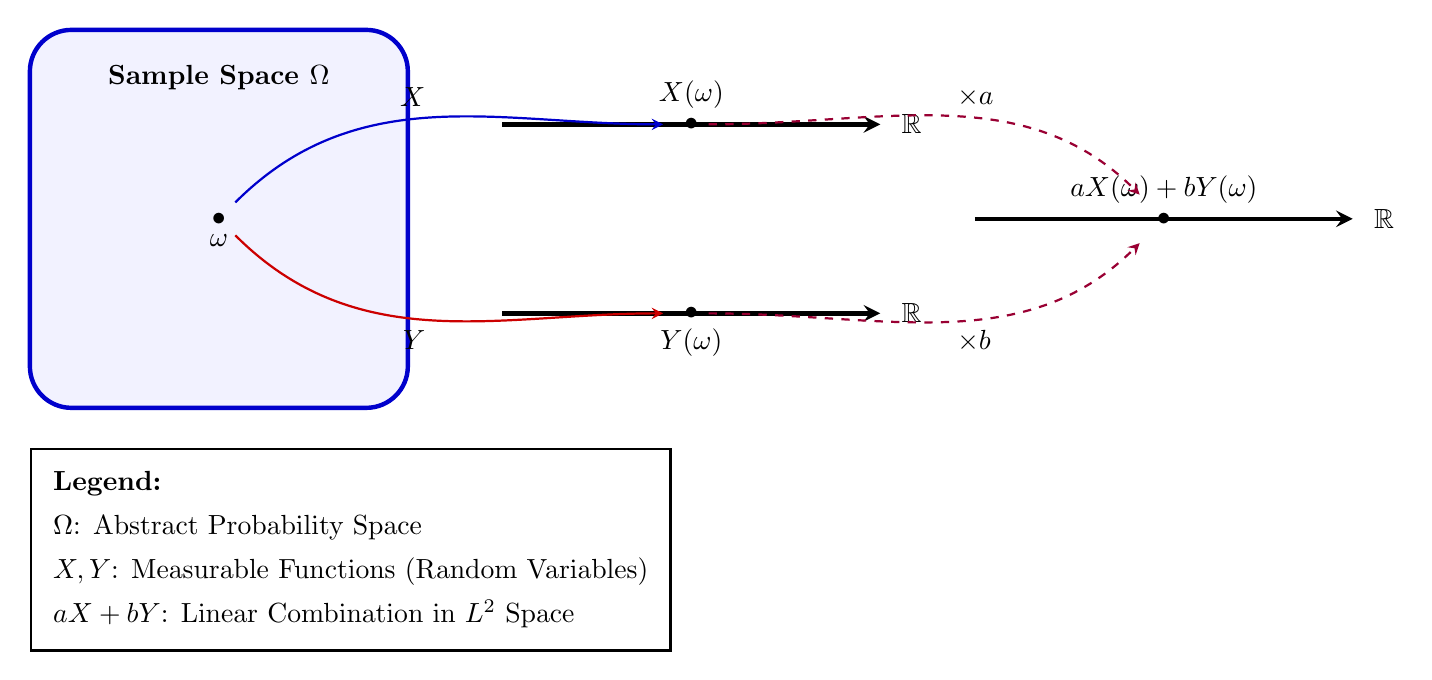
\begin{tikzpicture}[scale=1.2, >=stealth, thick]
    % 1) Backgrounds
    \fill[blue!5, rounded corners=15pt] (-2, -2) rectangle (2, 2);
    
    % 2) Axes / Grids
    \draw[blue!80!black, ultra thick, rounded corners=15pt] (-2, -2) rectangle (2, 2);
    
    % 3) Primary Plots / Mappings
    \draw[->, ultra thick] (3, 1) -- (7, 1);
    \draw[->, ultra thick] (3, -1) -- (7, -1);
    \draw[->, ultra thick] (8, 0) -- (12, 0);
    
    % 4) Nodes and Labels
    \node[black, font=\bfseries] at (0, 1.5) {Sample Space $\Omega$};
    \node[black] (omega) at (0,0) {$\bullet$};
    \node[black, below=2pt] at (omega) {$\omega$};
    
    \node[black] (x_val) at (5, 1) {$\bullet$};
    \node[black, above=2pt] at (x_val) {$X(\omega)$};
    \node[black, right=4pt] at (7, 1) {$\R$};
    
    \node[black] (y_val) at (5, -1) {$\bullet$};
    \node[black, below=2pt] at (y_val) {$Y(\omega)$};
    \node[black, right=4pt] at (7, -1) {$\R$};
    
    \node[black] (z_val) at (10, 0) {$\bullet$};
    \node[black, above=2pt] at (z_val) {$aX(\omega) + bY(\omega)$};
    \node[black, right=4pt] at (12, 0) {$\R$};
    
    % Arrows
    \draw[->, blue!80!black, shorten >=4pt] (omega) to[out=45, in=180] node[above left, black] {$X$} (x_val);
    \draw[->, red!80!black, shorten >=4pt] (omega) to[out=-45, in=180] node[below left, black] {$Y$} (y_val);
    
    \draw[->, purple!80!black, dashed, shorten >=4pt] (x_val) to[out=0, in=135] node[above right, black] {$\times a$} (z_val);
    \draw[->, purple!80!black, dashed, shorten >=4pt] (y_val) to[out=0, in=-135] node[below right, black] {$\times b$} (z_val);
    
    % Legend
    \node[align=left, inner sep=8pt, draw=black, fill=white, anchor=west] at (-2, -3.5) {
        \textbf{Legend:}\\[4pt]
        $\Omega$: Abstract Probability Space\\[4pt]
        $X, Y$: Measurable Functions (Random Variables)\\[4pt]
        $aX+bY$: Linear Combination in $L^2$ Space
    };
\end{tikzpicture}
\end{center}

\subsection{Heuristics \& "Cheats"}
\begin{itemize}
    \item \textbf{The "Square the Constant" Rule:} Never pull a constant out of a variance operator without squaring it. $V(-X) = (-1)^2 V(X) = V(X)$.
    \item \textbf{The Independence Shortcut:} If a problem explicitly states variables are independent, immediately cross out the covariance term in your variance expansion. It saves time and prevents algebraic errors.
\end{itemize}

\subsection{Pitfalls \& Fallacies}
\begin{itemize}
    \item \textbf{The Zero-Covariance Fallacy:} Assuming that $\text{Cov}(X,Y) = 0$ implies $X$ and $Y$ are independent. This is false. Independence implies zero covariance, but the converse is only guaranteed for jointly normal distributions.
    \item \textbf{Linearity of Non-Linear Operators:} Assuming $\E[X/Y] = \E[X]/\E[Y]$ or $\E[X^2] = (\E[X])^2$. Expectation is strictly a linear operator.
\end{itemize}

\newpage
\section{Part 5: Conceptual Synthesis and The "Big Picture"}

\subsection{A) Thematic Connections}
The central theme of this topic is the \textit{vector space structure of random variables}. If we consider random variables with finite second moments, they form a Hilbert space known as $L^2(\Omega, \F, \Prob)$. In this space, the covariance acts as an inner product: $\langle X, Y \rangle = \text{Cov}(X, Y)$. 
Theorem 5.12 is simply the probabilistic equivalent of the geometric Law of Cosines: $\|aX + bY\|^2 = a^2\|X\|^2 + b^2\|Y\|^2 + 2ab\langle X, Y \rangle$. This unifies abstract linear algebra with measure-theoretic probability.

\subsection{B) Forward and Backward Links}
\textbf{Backward Links:} This topic relies heavily on the double integration techniques from multivariate calculus to find marginals and covariances, bridging deterministic calculus with stochastic modeling. \\
\textbf{Forward Links:} Understanding the variance of sums is the absolute prerequisite for the \textbf{Central Limit Theorem (CLT)}. The CLT relies on the fact that the variance of the sample mean $\bar{X}$ scales by $1/n$, which we proved using Theorem 5.12. Furthermore, this forms the foundation for Stochastic Calculus (Ito's Lemma) where we analyze linear combinations of Brownian motion increments.

\section{Part 6: Abstract Real-World Modeling (AI, ML, \& Quant Finance)}

\subsection{A) Concrete Scenarios}
\begin{enumerate}
    \item \textbf{Quantitative Finance (Markowitz Portfolio Theory):} An investor wants to allocate capital across $N$ volatile assets. The portfolio return is a linear combination of individual asset returns. Theorem 5.12 is used to calculate the portfolio's total risk (variance), allowing the investor to minimize risk through diversification (negative covariances).
    \item \textbf{Machine Learning (Random Forests):} In ensemble learning, a Random Forest averages the predictions of $N$ decision trees. If the trees are highly correlated, the variance of the ensemble remains high. By forcing the trees to be de-correlated (via random feature selection), the covariance terms in Theorem 5.12 drop, drastically reducing the model's overall variance and preventing overfitting.
\end{enumerate}

\subsection{B) Model Problem Setup: Markowitz Portfolio Optimization}
Let the state space be the financial market with $N$ assets. Let $R = (R_1, R_2, \dots, R_N)^T$ be the random vector of asset returns, defined on probability space $(\Omega, \F, \Prob)$.
Define the mean return vector $\mu = \E[R]$ and the positive-definite covariance matrix $\Sigma = \E[(R-\mu)(R-\mu)^T]$.
Let $w = (w_1, w_2, \dots, w_N)^T$ be the deterministic vector of portfolio weights, subject to the budget constraint $\sum w_i = 1$.
The portfolio return is a linear combination: $U = w^T R = \sum_{i=1}^N w_i R_i$.
By Theorem 5.12, the expected return is $\E[U] = w^T \mu$, and the portfolio variance (risk) is:
\[ V(U) = w^T \Sigma w = \sum_{i=1}^N w_i^2 V(R_i) + 2 \sum_{1 \le i < j \le N} w_i w_j \text{Cov}(R_i, R_j) \]
The quantitative optimization problem (a Quadratic Program) is to find the weights $w$ that minimize risk for a target return $\mu^*$:
\[ \min_{w} \frac{1}{2} w^T \Sigma w \quad \text{subject to} \quad w^T \mu = \mu^* \quad \text{and} \quad w^T \mathbf{1} = 1 \]
This rigorous application of Theorem 5.12 is the foundation of modern algorithmic trading and risk management.

\newpage
\section{Part 7: Common Variations and Untested Concepts}

\subsection{Quadratic Forms of Random Variables}
While the homework thoroughly covers linear combinations, advanced courses frequently test \textit{quadratic forms}. A quadratic form is an expression of the type $U = X^T A X$, where $X$ is a random vector and $A$ is a deterministic symmetric matrix. This appears heavily in multivariate statistics and machine learning (e.g., Mahalanobis distance).

\textbf{Theorem:} Let $X$ be a random vector with mean $\mu$ and covariance matrix $\Sigma$. Let $A$ be a symmetric matrix. Then:
\[ \E[X^T A X] = \text{tr}(A \Sigma) + \mu^T A \mu \]
where $\text{tr}(\cdot)$ denotes the trace of a matrix.

\textbf{Rigorous Proof:}
Since $X^T A X$ is a scalar, it is equal to its own trace. We use the cyclic property of the trace operator, $\text{tr}(ABC) = \text{tr}(CAB)$, and the linearity of expectation.
\begin{align*}
\E[X^T A X] &= \E[\text{tr}(X^T A X)] \\
&= \E[\text{tr}(A X X^T)] \\
&= \text{tr}(A \E[X X^T])
\end{align*}
By the definition of the covariance matrix, $\Sigma = \E[(X-\mu)(X-\mu)^T] = \E[X X^T] - \mu \mu^T$.
Therefore, the uncentered second moment matrix is $\E[X X^T] = \Sigma + \mu \mu^T$.
Substituting this back:
\begin{align*}
\E[X^T A X] &= \text{tr}(A (\Sigma + \mu \mu^T)) \\
&= \text{tr}(A \Sigma) + \text{tr}(A \mu \mu^T) \\
&= \text{tr}(A \Sigma) + \mu^T A \mu
\end{align*}
This completes the proof. $\blacksquare$

\newpage
\section{Part 8: Advanced Diagnostic Testing: "Find the Flaw"}

Below are five advanced proofs/solutions containing a single, subtle logical flaw. 

\textbf{Problem 1:} Let $X$ and $Y$ be random variables with $V(X)=4$ and $V(Y)=9$. We wish to find the variance of their difference. By the properties of variance, $V(X-Y) = V(X) - V(Y) = 4 - 9 = -5$.

\textbf{Problem 2:} Let $X$ be a standard normal random variable, $X \sim N(0,1)$. We want to find the variance of the scaled variable $3X$. Using the linearity of the variance operator, $V(3X) = 3V(X) = 3(1) = 3$.

\textbf{Problem 3:} Let $X$ be a random variable uniformly distributed on $[-1, 1]$. Let $Y = X^2$. We calculate the covariance: $\text{Cov}(X,Y) = \E[XY] - \E[X]\E[Y] = \E[X^3] - (0)\E[Y] = 0 - 0 = 0$. Since the covariance is zero, $X$ and $Y$ are independent random variables.

\textbf{Problem 4:} Let $X$ and $Y$ be independent uniform random variables on $(0,1)$. We want to find the expected value of their ratio, $\E[X/Y]$. By the linearity of expectation, $\E[X/Y] = \E[X] / \E[Y] = (1/2) / (1/2) = 1$.

\textbf{Problem 5:} Let $X_1, X_2, \dots, X_n$ be independent random variables drawn from a Cauchy distribution. Let $\bar{X} = \frac{1}{n}\sum X_i$ be the sample mean. By Theorem 5.12, $V(\bar{X}) = \frac{1}{n^2} \sum V(X_i) = \frac{1}{n} V(X_1)$. As $n \to \infty$, the variance of the sample mean approaches 0, proving the Law of Large Numbers for the Cauchy distribution.

\vspace{2em}
\hrule
\vspace{1em}
\subsection*{Solution Key: Resolutions to the Flaws}

\textbf{Resolution 1:} Variance is a measure of dispersion and must always be non-negative. The flaw is assuming $V(X-Y) = V(X) - V(Y)$. The correct formula is $V(X-Y) = V(X) + V(Y) - 2\text{Cov}(X,Y)$. Even if they are independent, the variances add: $4 + 9 = 13$.

\textbf{Resolution 2:} The variance operator is not linear; it is quadratic. When pulling a constant out of a variance operator, it must be squared. The correct step is $V(3X) = 3^2 V(X) = 9(1) = 9$.

\textbf{Resolution 3:} The flaw is the logical fallacy of Affirming the Consequent. While independence implies zero covariance, zero covariance does \textit{not} imply independence. Here, $Y = X^2$, meaning $Y$ is completely deterministically dependent on $X$, despite having zero covariance (they have a non-linear relationship).

\textbf{Resolution 4:} The linearity of expectation applies strictly to sums, not quotients. The correct step utilizes independence: $\E[X/Y] = \E[X \cdot (1/Y)] = \E[X]\E[1/Y]$. However, $\E[1/Y] = \int_0^1 (1/y) \, dy = \infty$. The expectation does not exist.

\textbf{Resolution 5:} The flaw is a violation of the foundational assumptions of Theorem 5.12. The theorem requires the random variables to have finite second moments. The Cauchy distribution has undefined (infinite) variance and mean. Therefore, Theorem 5.12 cannot be applied, and the sample mean of Cauchy variables does not converge to a constant; it remains Cauchy distributed.

\end{document}